\documentclass{beamer}
\usetheme{Warsaw}

\usepackage[utf8]{inputenc}
\usepackage{fancybox}
\usepackage{multimedia} 
\usepackage{subfig}
\usepackage{amsmath}

\usepackage[all]{xy}
\begin{document}


\title[Computergrafik] % (optional, only for long titles)
{Computergrafik

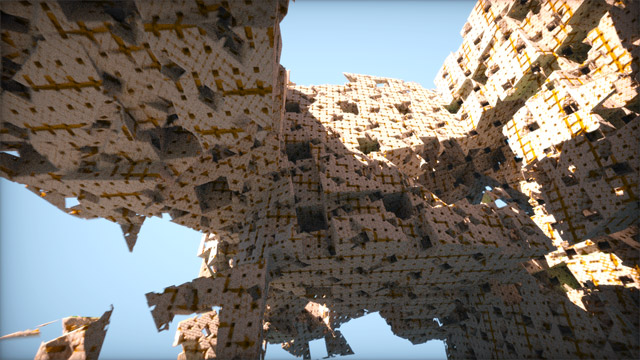
\includegraphics[scale=0.36]{images/cover}
}
\subtitle{}
\author[Dr. Johannes Riesterer] % (optional, for multiple authors)
{Dr.  rer. nat. Johannes Riesterer}

\date[KPT 2004] % (optional)
{}

\subject{Computergrafik}




\begin{frame}
    \frametitle{Computergrafik}
\framesubtitle{}
    \begin{block}{Echzeit Darstellung}
Kombination von Soft- und Hardware
\end{block}
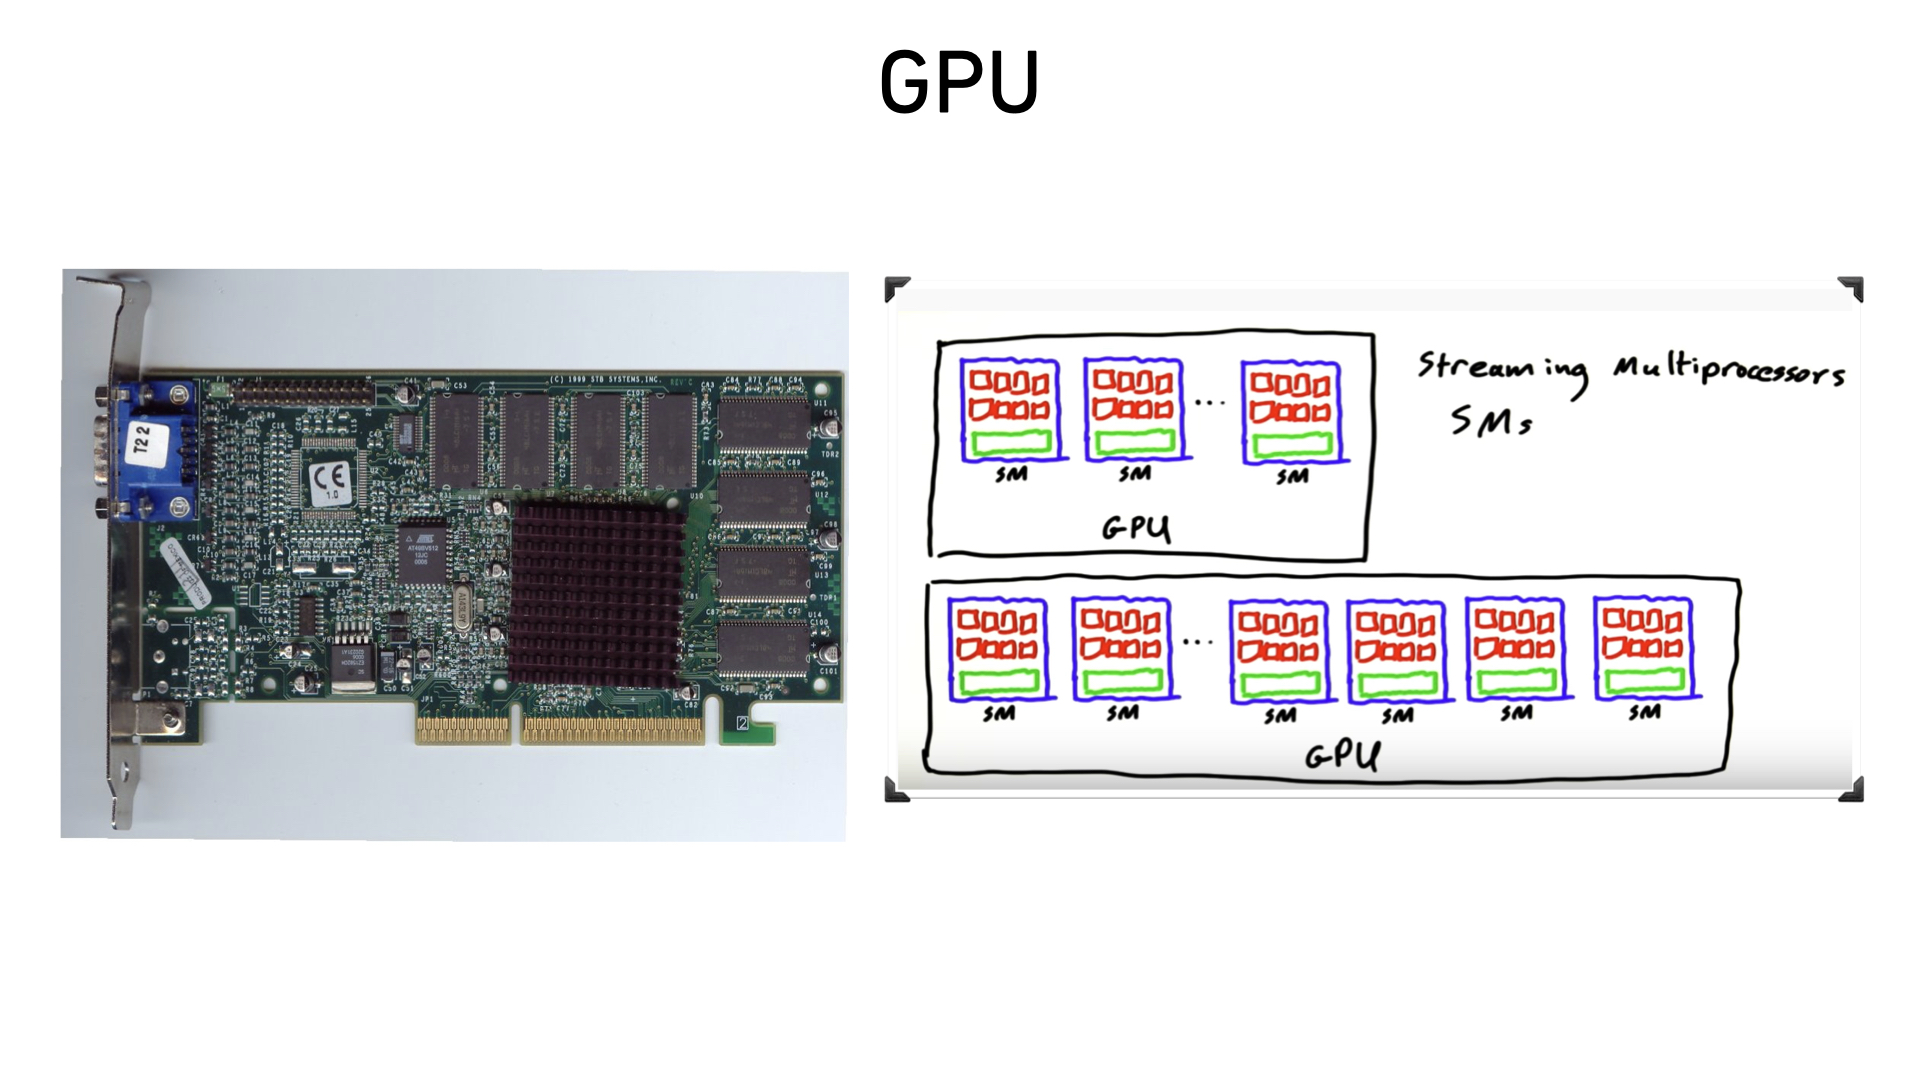
\includegraphics[scale=0.1]{images/Shaderday_Intro/Shaderday_Intro_004} \\
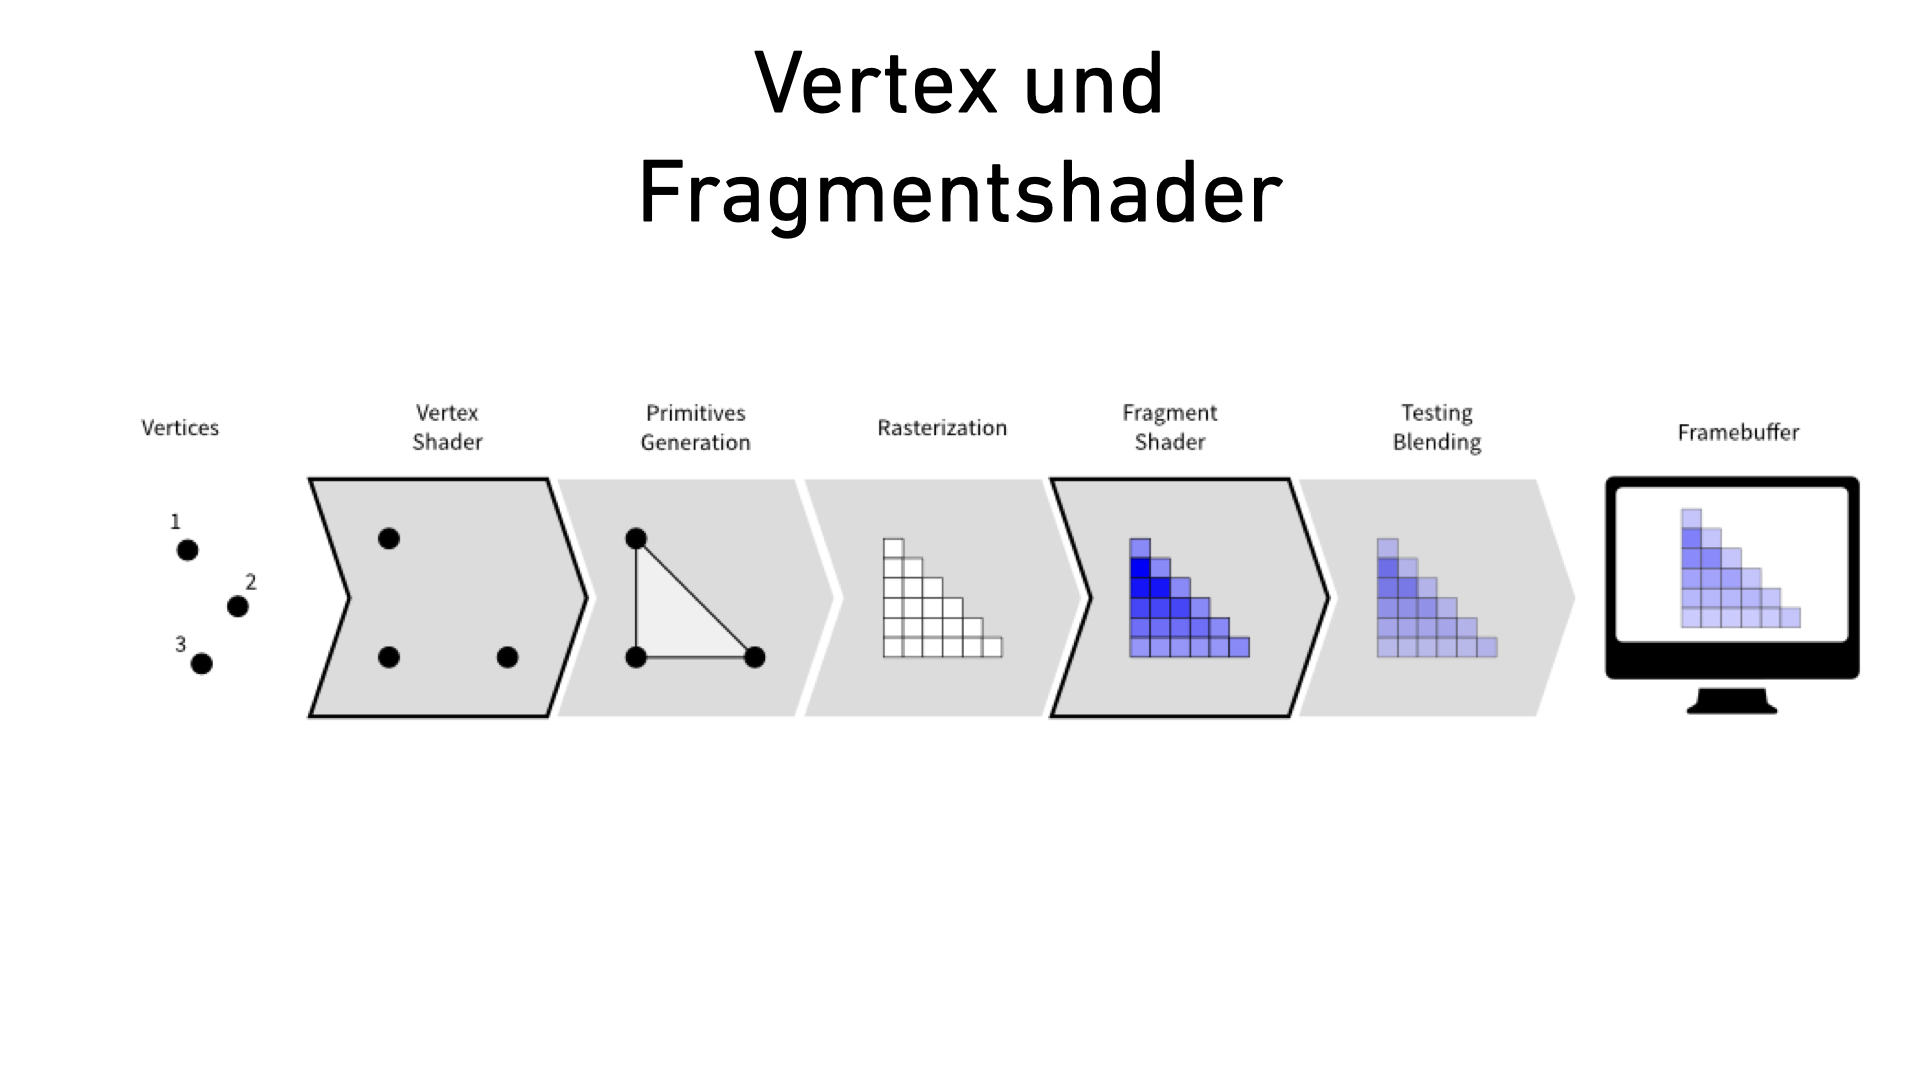
\includegraphics[scale=0.1]{images/Shaderday_Intro/Shaderday_Intro_007}

\end{frame}


\begin{frame}
    \frametitle{Computergrafik}
\framesubtitle{}

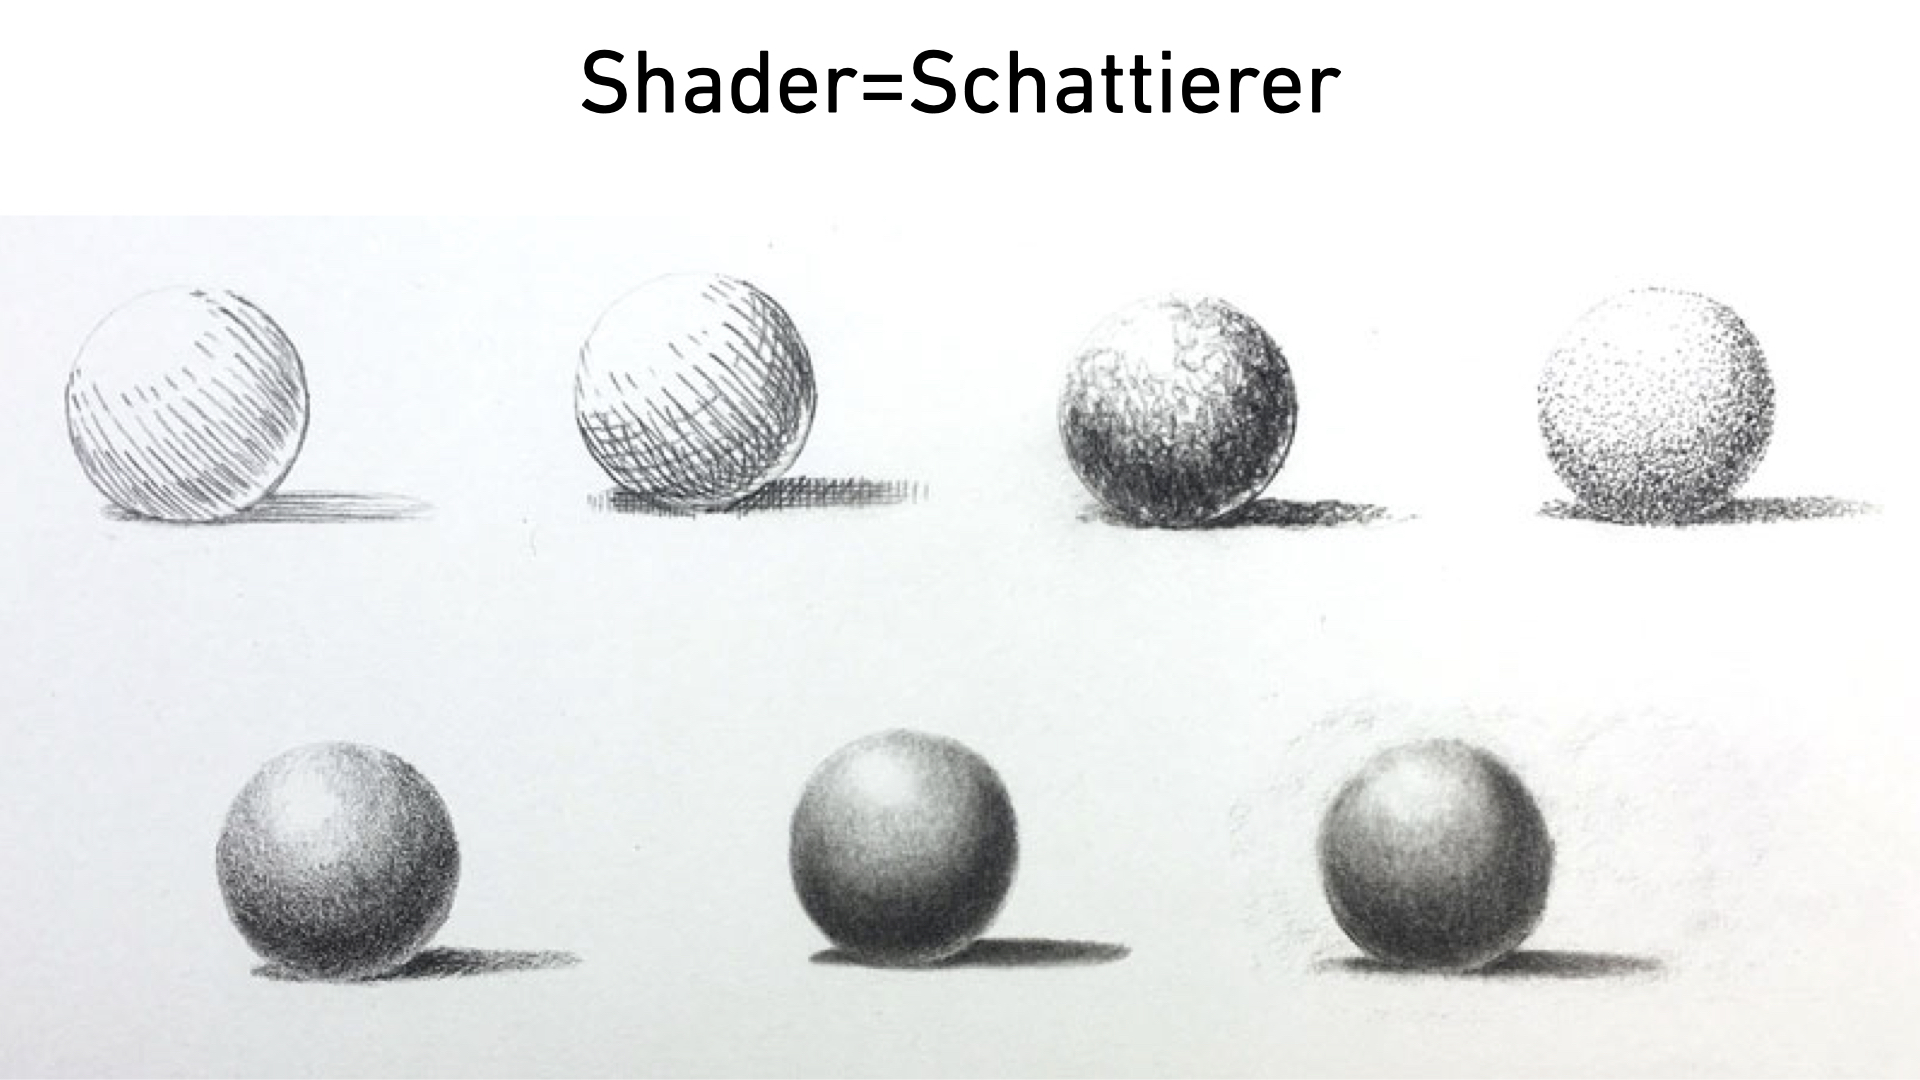
\includegraphics[scale=0.12]{images/Shaderday_Intro/Shaderday_Intro_001} 
\end{frame}



\begin{frame}
    \frametitle{ Shaderprogramm}
\framesubtitle{}
\begin{center}
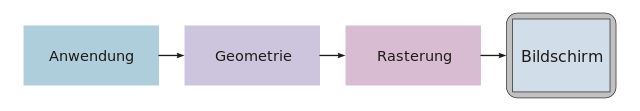
\includegraphics[scale=0.26]{images/cgpipeline_grob}
\\
\includegraphics[scale=0.20]{images/Zeichnung_Shaderpipeline}

\end{center}
\end{frame}

\begin{frame}
    \frametitle{OpenGL Pipeline}
\framesubtitle{}
    \begin{block}{}
\begin{center}
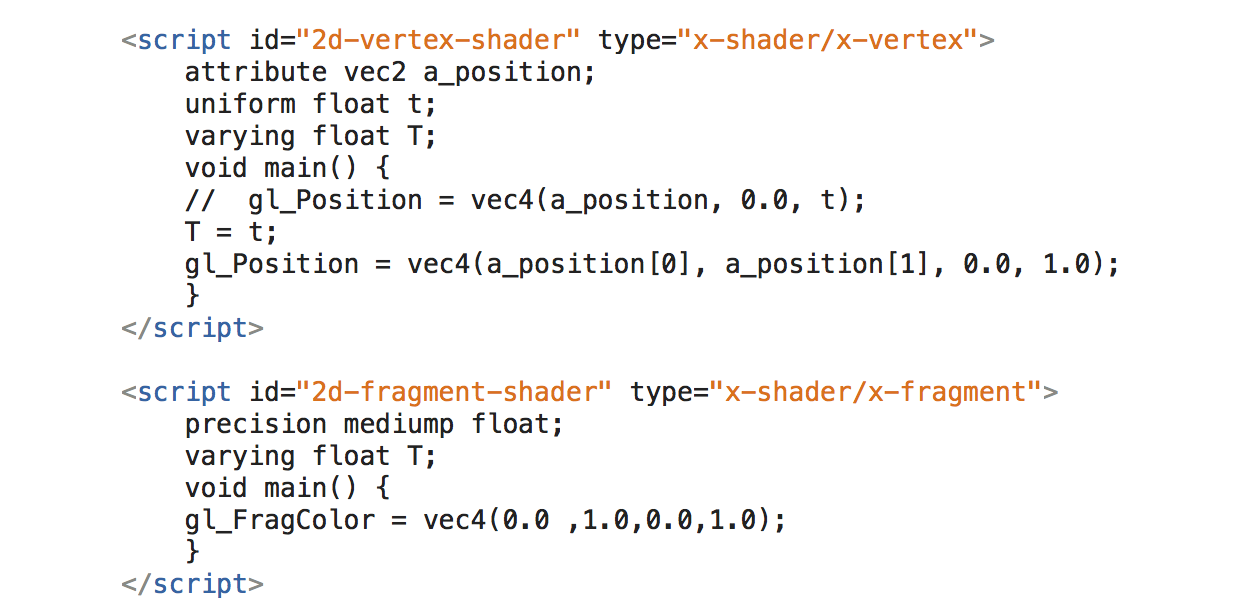
\includegraphics[scale=0.56]{images/shader}
\end{center}
\end{block}
\end{frame}



\end{document}
